\chapter{Working plan}
%\thispagestyle {empty}
\section{Description and objectives}

	An open source multi-platform management application for high school teachers is developed. It can be run on a smartphone or tablet. 
	The actual objectives of the application are students management:
	\begin{itemize}
	  \item Attendance and punctuality control. 
	  \item Misbehaviour control.
	  \item Activities assessment. Each student will have an activity mark.
	\end{itemize}

	Application would also include these features:
	\begin{itemize}
	  \item Data visualization. As table-like format. Attendance and misbehaviour
	  \item Server synchronization with a custom application or Xade \cite{Xade}.
	\end{itemize}

	The final goal is to develop an application to make teacher's work easier and comfortable. This application is focused on user  (teacher) experience.
	Also an objective is to write extensible, easy to read code, which allows external developers to take part into application development.
	
	Below, a list of tasks to be done to fullfil application development:
	\begin{itemize}
	  \item Study state-of-art solutions: 
  \subitem  Find out other solutions: PDAs and smart-phone or tablet related and web-based applications.
  \subitem  Download to study and reuse graphical user interfaces, code or/and database structure. 
  \item   Develop database structure: tables (field names and type of data), and relationships among tables. 
  \item   Preparation for development:
\subitem  Build development and staging environment: 
\subsubitem Install Eclipse \cite{Eclipse}, Android Virtual Machine \cite{AndroidDevelopmentKit}, Aptana Plugin for Eclipse, JQuery, JQueryMobile \cite{JQueryMobile} and Phonegap \cite{PhoneGap} from their respective websites \cite{PhoneGapGS}.
\subitem   Choose application name and folder's policy.
\subitem   Make a simple application: only a blank page.
\subitem  Configure a git repository and upload the application: \cite{EduXes}.
	\end{itemize}
	
		
  Development will follow these stages:
	\begin{itemize}
  \item   Populate database with sample data. Firstly, data will be hard-coded into source code to stagging. Several tables will be created:
  groups, students, sessions, teacher schedule, students attendance, activities, student activities, and activities per group. Secondly 
  the appropiate windows to manage these tables will be built.
  
  \item   Groups: Several groups (four) of students will be hard-coded into javascript source code, with three or four students each other.
  \subitem  Make list of groups window. This will list the four groups.
  \subitem  Groups management window. Another group could be added, or removed.
  
  \item  Students information:
  \subitem   Make list of students window per group and complete list of students. 
  \subitem   Students management window: to insert and update data students: name, surname, birthday, address, e-mail,  tutor name,
    landline and cell phone numbers and nationality.
    
  \item  Sessions. Each lecture has a description (as 'first hour', or 'recreation'), starting and ending time.  These sessions will be hard-coded on first version.
  \item  Teacher schedule. For the current teacher, it contains weekly and daily schedule: name of group, session and day of the week. This information will be also hard-coded. 
  \item Main window (or \emph{page} in PhoneGap notation) will be created. Teacher can set current data and go to \textit{daily page}, 
   manage activities, students and groups or manage reports: assessment and attendance. Next page will be \textit{daily page}.
   
  \item Timetable for current date: daily schedule, list of groups for each day ordered by session.
  
  \item Attendance page will be next to be build. It contains a list of students by group. Teacher can assign an attendance code to each student (attendance, misbehaviour, unpunctuality or excused).
  
  \item Assessment page is next to previous one. It contains one upper list of activities and a list of students similar to 
  \emph{attendance page }. Teacher could set activity and assign adequate mark to each student.
     
  \item  Activities. This page manage activities (add and disable activities \footnote{still not coded} ): name and description of assessable exercises. 
  \subitem  Activities group will be set in activities page, and activities student will be related with assessment.
  \item Reports pages.
  \subitem  List activities.
  \subitem  List groups.
  \subitem  List students by group.
  \subitem  List students attendance by week. User can select previous or next week, or set another date.
  \subitem  List students marks and final mark.
  
  \item Error handling. While developing each SQL query, any error will be catched and an error window will appears. 
  \item Eventually, test into real hardware: an Android 2.3.3 mobile phone, tablets, and so on.
  \end{itemize}
  
	   Next steps will include :  
  \begin{itemize}
  \item   Load data from an external file. This is well-documented \cite{PhoneGapLS}.  
  \item   Load images from disk (SD-Card).
  \item  Save or download data from database to disk.
  \item  Xade web interface.
  \subitem    a) Study Xade web interface.
  \subitem    b) Develop an ad-hoc application for retrieve Xade's data. With javascript or a native one. 
  \subitem    8. Develop an ad-hoc application for store data. 
  \subitem    9. Synchronization with a custom server or with Xade.
  \item   Test units. To ensure previous step were implemented.
  \item   User documentation. Manual with images.
  \item   Developer's documentation.
  \item   Find out a website to host a forum, a bug report system,  documentation and application download.
	\end{itemize}

Task above could be achieved in a 300 hour basis.	
In the following table a broad estimation of time spent in each task are shown.  


\begin{tabular}{lc}
Task    & Time (hours) \\
\hline 
State-of-art solutions   & 10 \\
Develop database & 8 \\
Preparation for development & 40 \\
Development.  & \\
\cr
	Populate database with sample data. & 20 \\
	Groups. List and management & 50 \\
	Students. List and management. & 30 \\
	Timetable for current date. & 80 \\
	Add attendance, behaviour. & 50 \\
	Add error handling. &2 \\
	Retrieve and insert data from and to database. &30 \\
	List of attendance, misbehaviour incidents. &12 \\
	Add activities grades for each student. &12 \\
	List students marks and final mark. &14 \\
	Activities management window.  &14 \\
	Management of student notes. &20 \\
	List of student notes.  &2 \\
Test into real hardware &20 \\
\hline
Total &384 \\
\end{tabular}

\section {Motivation}
  As a Technologies teacher, in my daily work I have to evaluate students work such as working with tools, cooperative work with other classmates etc., besides usual activities as written exercises. A long data sheet could used, or an awkward long spreadsheet, but a portable device with a custom application should be desirable.
  
	This application tries to increase teacher's productivity because teacher only has to write attendance, or unpunctuality two times (on official report and on application's window), and classroom notes and activity grades on very easy way.
	
	The most important feature is to be as easy, fast and intuitive as possible. It could be desirable to be platform independent (Android, iOS, Windows RT), but Android is preferred because it is open source and has a higher market share.
	
	On the other hand, development of this application improves my computer science skills in  mobile-phone applications development: JQuery,  jQueryMobile, PhoneGap/Cordova, SQLite, Android,  git repository management.

\section {Methodology \label{Methodology}}
	This work was carried on building small blocks, also called pages, and make it up into final application.
	A page is a visible window, only first page is visible, and other pages are called from this one.
	
	 Database structure was separated from interface, and interface was also separated into dynamic and static contents. Each new
	 functionality was written, tested, and
	polished. 
	
	Foremost a new window/page is designed from previous HTML code or from sample code \cite{SergasApp} and written
	in {\bf index.html} , \emph{id} are set with ad-hoc names  (e.g. \emph{id="edit\_student"}, 
	   \emph{id="in\_name\_student"}),   these \emph{id's} are used in javascript code. 
	   
	   
	%% logo=\bcrayon,
\begin{bclogo}[couleur=blue!30,arrondi=0.1,ombre=true ] 
%% \begin{bclogo}[couleur=blue!30,arrondi=0.1, logo=\bcpanchant, barre=zigzag,  ombre=true ] 
{Sample Page. index.html}
\begin{verbatim}
<div data-role="page" id="daily\_work">
    <div data-role="header" data-add-back-btn="true" data-theme="a">
                <h1>Day</h1>
    </div>
    <div data-role="content" data-theme="a">
        <div class="ui-grid-b">
            <div class="ui-block-a">
                <div data-role="fieldcontain">
                    <label for="date"  >Date:</label>
                </div>
            </div>
            (...)
        </div>
    </div>
    <div data-role="navbar">
        <ul>
            <li>
                <a href="#" onClick="onGeneralFile()"  
                data-role="button" data-icon="star"  
                data-theme="a" > File</a>
            </li>
            <li>
            (...)
            </li>
        </ul>
    </div><!-- /navbar -->
    <div data-role="footer" class="footer-docs" data-theme="a">
        <p   style="text-align:center;"  id="teachers\_name"></p>
    </div>
</div> 
\end{verbatim}

\end{bclogo}
	   
	   
	   
	   
	   
    Secondly { \bf interface.js} code are written: show progress icon (a \emph{PhoneGap} function), a customized function which loads data into new HTML code (e.g. \emph{loadGroupAssessment}) , 
    and, finally a \emph{PhoneGap} function to  show new page/window.
\begin{bclogo}[couleur=blue!30,arrondi=0.1,ombre=true ] 
{Sample interface.js code}        
        \begin{verbatim}
$.mobile.showPageLoadingMsg();
id_group=global_id_group; 
loadGroupAssessment(global_db,id_group);
$.mobile.changePage("#list_students_assessment");
    \end{verbatim}  
\end{bclogo}

    Thirdly {\bf database.js} code are written: Declaration of previous function \ref{function1}, which  usually implements a SQL-query to SQLite database. These functions also fill html code, so HTML \emph{id}'s names are so significant.
    
\begin{bclogo}[couleur=blue!30,arrondi=0.1,ombre=true ] 
{Sample database.js code}    
\begin{verbatim}
var list_asset=$('#list_assessment_select'); 
sql="SELECT ";
sql += " ACTIVITIES_GROUP.a_date (...)  ";

db.transaction(function(tx) {
    tx.executeSql(sql,[],
        dbSuccessFunc = function(tx, results) {
           var html ="";
           for (var i=0;i<results.rows.length;i++) {
              a_id = results.rows.item(i).a_id;
              a_name = results.rows.item(i).a_name;
                    (...)
              html +=' <option value="'+a_id+'">'+a_name+'</option> ';
           }
           list_asset.empty().append(html);
           list_asset[0].selectedIndex = 0; 

           if(results.rows.length>0) {
             $('#current_group_assessment').text(
                results.rows.item(0).g_data); 
           }
           global_id_group = id_group;
           listStudentsByGroupAssessment( db, id_group, 
            $('#students_assessment_ul'));
       },
       dbErrorFunc (...)
        ); 
});
\end{verbatim}    
\end{bclogo}    
    
    After successful tests using Android Emulator provided by Android SDK \cite{AndroidDevelopmentKit}, {\bf TODO} file could be updated, and code will be upload to remote git \cite{EduXes} repository.
  
  \begin{bclogo}[couleur=green!30,arrondi=0.1, logo=\bcpanchant,  ombre=true ] 
{Git init shell}   
\begin{verbatim}
$ git add -A *
$ git commit -m BRIEF_DESCRIPTION_OF_CHANGES 
$ git push origin master
\end{verbatim}
\end{bclogo}

	  From time to time application is downloaded from git repository into real hardware and tested. It is usually faster on 
	  a mobile-phone than on emulator. 
	    
		\section{Tools}
	
	Tools involved in \emph{EduXes} development are :
	\begin{itemize}
	    \item IDE. Eclipse \cite{Eclipse}. The most popular Integrated Development Environment for Java and other languages. 
	    It integrates  browser, contextual help, even Android Virtual Machine is integrated.
	    \item Aptana \cite{Aptana}. Aptana Plugin is used  HTML, CSS and JavaScript editing. 
	    \item Android Development Kit \cite{AndroidDevelopmentKit}.  Android SDK provides  the API libraries and developer tools necessary to build, test, and debug apps for Android.  
	    \item Git. Also included as an Eclipse plugin.
	\end{itemize}

	


	
\section {Work plan}

Following previous methodology \ref{Methodology}, a detailed plan is shown below:
\begin{itemize}
    \item {HTML}. User interface. 
    \item {interface.js}. Functional code and database agnostic.
    \item {database.js}. Database related code.
    \item {DATABASE.sql}. Database declarations as a standalone file.
\end{itemize}

    
	\subsection{HTML}
  There are only two html files: \textbf{index.html} and \textbf{remove.html}. The most important: \textbf{index.html} file is build by
   blocks called pages, gathered together \cite{JQueryMobilePage}. Each page is its own {\bf div } 
   with custom properties (\emph{propieraty} properties in Eclipse jargon ) : {\bf data-role="page"}. Below as show an example: list of several reports, user could choose one and a function (\emph{onReportListAttendance() } or \emph{onReportListAssessment() }  ) is executed .
   
   
  Inside each page there are several identificatives \emph{id="name"} which are used by application to fill with data (e.g.
   within \emph{daily\_schedule} page \emph{current\_day} id is used to set date to current date). 
  
\begin{bclogo}[couleur=blue!30,arrondi=0.1,ombre=true ] 
{Reports Page}
\begin{verbatim}
  
 <div data-role="page" id="list_reports" data-add-back-btn="false">
            <div data-role="header"  data-back-btn-text="previous" 
              data-add-back-btn="false" >
            <a href="#daily_work"  data-icon="arrow-l" data-theme="a" 
              data-role="button">Back</a>
                <h1>Reports</h1>
            </div>
            <div data-role="content">

                <ul data-role="listview" id="list_reports_ul" 
                  data-split-icon="gear" data-split-theme="a" 
                  data-filter="false" 
                  data-inset="true" data-theme="a" >
                <li><a href="#" onClick="onReportListAttendance();"
                 >Attendance</a></li>
                <li><a href="#" onClick="onReportListAssessment();" 
                >Assessment</a></li>
                <li><a href="#" onClick="" >File</a></li>
                </ul>
            </div>
            <div data-role="footer" class="footer-docs" 
                data-rel="back"
             data-theme="a">
             </div>
 </div>
\end{verbatim}

\end{bclogo}

A complete list of pages is shown below:

\begin{bclogo}[couleur=orange!30,logo=\bcbook,arrondi=0.1,ombre=true ] 
{List of Pages}
\begin{tabular}{l|l}
intro & Introductiony page              \\
daily\_work & daily work \\
list\_reports & List reports             \\
list\_settings  & List settings\\
file & Exit application                  \\
daily\_schedule & List of groups per day\\
list\_students\_attendance &             \\
list\_students\_assessment &  \\
list\_students\_attendance\_by\_group &  \\
general\_list\_attendance &  \\
list\_groups\_attendance  &              \\
list\_groups\_assessment &  \\
list\_students\_assessment\_reports &    \\
list\_groupsto\_edit &  \\
edit\_new\_group &                      \\
 edit\_groups  & \\
list\_groups &                          \\
  list\_students\_by\_group & \\
list\_students &                        \\
  edit\_student   &   \\
edit\_new\_student &                    \\
  list\_all\_activities & \\
update\_activity  &                     
\end{tabular}

\end{bclogo}	

	
	\subsection{Interface code }
	There is only onle file which deals with interface interactions (events from {\bf html} files): \emph{ interface.js}.
If the function is called directly from \emph{html}	code, function name contains {\bf on} prefix.
There are several groups of functions:
\begin{itemize}
    \item \emph{Students} and \emph{Groups} functions, which manage and list general students and groups information.
    \item \emph{Activities} functions, which update, list and add new activities.
    \item \emph{Assessment} functions, list and update students marks.
    \item \emph{Attendance} functions, list when student attend classes and update their values.
\end{itemize}
Whether these functions need access to data (every function but \emph{ onGeneral* } ) they call  their counterpart 
function in {\bf database.js } file.

\begin{bclogo}[couleur=orange!30,logo=\bcbook, arrondi=0.1,ombre=true ] 
{List of Functions: {\bf interface.js}}	
\begin{tabular}{lll}
Name                    & Task            & Group \\
\hline
\emph{ onDeviceReady()  }&  Firstly loaded, create and    &  Initial\\
&populate database,              &                          \\
&load initial page               &                          \\
\emph{ init()  } &Initial                         &   \\
\emph{ initialize\_data ()      } &Load default date               &    Initial \\
\emph{ open\_daily\_page()     } &Daily work page:                &   Schedule \\
& list of groups                  &                           \\
\emph{ listStudentsAttendance() }&Students Attendance page        &   \\
\emph{ requestNewGroup()     }   & New Group                       &  Groups \\
\emph{ onAddNewGroup()       }   &Edit Group                      &   Groups \\
\emph{ onAddNewGroup()       }   &Update Group                    &  Groups \\
\emph{ onDeleteGroup()       }   &Delete Group                    &   Groups \\    
\emph{ onSaveNewGroup()      }   &Save Group                      &   Groups \\
\emph{ onListAllGroups()     }   &List All Groups                 &  Groups \\
\emph{ EditStudent()         }   &Edit Student                    &   Students \\
\emph{ onDeleteStudent()     }   & Delete Student                  &  Students \\   
\emph{ onAddNewStudent()     }   &Add new Student                 &   Students \\    
\emph{ onSaveStudent()       }   &Save Student                    &  Students \\
\emph{ onSaveNewStudent()    }   & Save New Student                &   Students \\
\emph{ listStudents()        }   & Full list of students           &  Students \\
\emph{ listStudentsByGroup( )}   & List Students by group          &  Students \\
\emph{ onListAllStudents()  }    & Full list of students           &  Students \\
\emph{ onListAllActivities()}   & List All Activities             &    Activities \\
\emph{ onUpdateActivity()  }   & Activity update                 &   Activities \\
\emph{ onAddNewActivity()  }   & Add new Activity                &   Activities \\
\emph{ onSaveNewActivity() }    & Save New Activity               &   Activities \\
\emph{ onOpenStudentsAssessment()} & Open Students Assessment        &   Assessment \\
\emph{ onRefreshGroupAssessment()} & Reload Group Assessment         &  Assessment \\
\emph{ onOpenStudentsAttendance() }& Open Student Attendance         & Attendance \\
\emph{ onReportListAttendance() }  & List Attendance                 &  Attendance\ \\
                         &                                   & Reports \\
\emph{ listStudentsByGroupAttendance() } & List Students by             & Attendance \\
    & Group Attendance           &    Reports \\
\emph{ studentsAttendanceListPrevious()} &List Students by Group     &  Attendance\\
    &Previous week                                              & Reports \\

\emph{ studentsAttendanceListNext()} & List Students by Group    & Attendance  \\
    &Next week   &   Reports\\

\emph{ onReportListAssessment() } & List Groups for Assessment      &   Assessment  \\
                         &                                   & Reports \\
  \emph{ onListStudentsAssessment()} & List Students for Assessment    &Assessment  \\
                         &                                   & Reports \\
 \emph{ studentState() }    & Student State       &   Student \\
\emph{ Attendance()}    & Student Attendance &   Student  \\
                 &                  &  Attendance \\
\emph{ onGeneralFile()} &Exit            &  Exit  \\
\emph{ onGeneralListReports()}    & List Reports    &  Reports \\
\emph{ onGeneralListSettings()}  & List Settings   &   Settings \\

\end{tabular}	
\end{bclogo}
	
	
	\subsection{Database code}
  The file which contains functions which carry on querys and data manipulation (on data base (SQLite)) is : \emph{ database.js}

There are  global variables on top of this file. These variables are used by functions because there are not obvious
ways to pass values from {\bf html } code  through functions ( e.g. as day week, database, current date, $\dots$ ):

  
\begin{shadowblock}{13cm}
\begin{tabular}{lc}
{\bf Variable}  & {\bf Meaning } \\
  \hline
  \texttt{global\_id}  & General and unique \\
                       & identification of any table   \\
                       & as students  \\                       
                       & or groups\footnote{will be deprecated} \\
\texttt{table\_global} & students, groups table\\

\texttt{global\_id\_group} &  Identification of a group \\
\texttt{global\_id\_student } &  Identification of a student \\
\texttt{global\_id\_activity} &  Identification of an activity  \\
\texttt{global\_max\_activities}& Number of activities \\
\texttt{global\_no\_groups} & Number of groups\\
\texttt{global\_week\_day} & Number of week day (0-6) \\
\texttt{global\_db }& Database pointer \\
\texttt{global\_session} &  Selected session \\
\texttt{global\_actual\_date} & Current date \\
\texttt{global\_reports\_date} & Date for reports\\

\texttt{global\_is\_new} & Whether activity is new \\

\texttt{global\_exist } & if exist current record\\

\texttt{STATE\_NONE  }& Default Student state\\
\texttt{STATE\_ABSENCE} & Truancy \\
\texttt{STATE\_UNPUNCTUAL}  & Unpunctuality \\
\texttt{STATE\_EXCUSED} & Excused unattendance  \\
\texttt{STATE\_BEHAVIOR } &  Bad behaviour \\

\end{tabular}
\end{shadowblock}

Several approaches have been considered, a lot of tiny, one function equals one simple task, but code were 
growing in complexity, became very difficult to read, maintain and pass variables to them. Other perspective was to write 
only several complete functions which carry all (or almost all) the work. From this point of view functions become longer, 
(up to a hundred of lines of code) but easier to test and follow.

Next tables list every function used in {\bf database.js}, gathered together by task, or menu options.

\begin{bclogo}[couleur=orange!30,logo=\bcbook, arrondi=0.1,ombre=true ] 
{List of Functions: {\bf database.js}}	
\begin{tabular}{ll}
Name                    & Task            \\
\hline
\emph{ errorCB() }                         & Error handler  \\
\emph{ successCB()            }           &  Success handler  \\

$\ulcorner$ \emph{ loadSchedule() }       & { Main Window $\rightarrow$ Load Daily Schedule } \\
\emph{ querySchedulePerDayDB() }         &  \\
$\llcorner $ \emph{ queryScheduleSuccess() }          &  \\
%%


$\ulcorner$ \emph{ loadAllStudents()}         &         Settings $\rightarrow $List all students \\
\emph{ queryAllStudentsDB() }             & \\
$\llcorner$\emph{ queryAllStudentsSuccess()}         &  \\

$\ulcorner$ \emph{ loadStudent()  }                  & Settings  $\rightarrow $List all students  $\rightarrow $ \\
              & Fill Students page\\
\emph{ queryStudentSuccess() }            &  \\
\emph{ queryStudentDB() }                 &  \\
%%
$\ulcorner$ \emph { loadNewStudent()   }     & {Settings $\rightarrow$ List all students $\rightarrow$ } \\
    &   New Student \\
$\llcorner$ \emph{ queryNewStudentDB() }              &  \\
%%
$\ulcorner$\emph{ loadStudents()  }                  & Delete Student $\rightarrow $List all students \\
 \emph{ queryStudentsDB() }                &  \\
$\llcorner$ \emph{ queryStudentsSuccess() }           &   \\





%%
\emph { loadStudentsByGroup()}          & { Settings  $\rightarrow$ Groups $\rightarrow$  List Students  } \\
%%
%%
%%
$\ulcorner$ \emph{ loadStudentAttendance()  }      &  Main Window $\rightarrow$ Load Daily Schedule  \\
                            &   $\rightarrow$ Groups (Default: Attendance)   \\

\emph{ queryStudentsAttendanceDB() }    & {  }\\
\emph{ queryStudentsAttendanceSuccess()}&    {   }\\
$\llcorner$\emph{ fillSelectStudent() }          & {  } \\
%%
$\lceil$ \emph { loadAllActivities() }           &{  Settings $\rightarrow$ Activities  } \\
$\llcorner$\emph { queryLoadAllActivitiesDB()}     &{   } \\
%%
\emph { loadActivity()}                & { Settings $\rightarrow$  Activities } \\
                                        & { List  $\rightarrow$ Load activity information } \\
\emph { updateActivity()}              &  { Settings $\rightarrow$ Activities }\\ 
                                       &  { List $\rightarrow$ Load activity } \\
                                       &  { $\rightarrow$ Update Activity. } \\
%
\emph { updateActivitiesGroup() }       & {idem. for each group } \\
%
\emph { insertNewActivity() }        & {Settings -> Activities -> New }\\
\emph { insertActivitiesGroup()}       & {idem. for each group } \\
%
\emph { loadGroupsActivitiesEdit( )}    & {Settings $\rightarrow$  Activities $\rightarrow$  New (List groups) } \\
%%
$\ulcorner$ \emph { listMaxActivities( ) }          &{ List Number of activities } \\
$\llcorner$ \emph { queryListMaxActivities() }      &{  } \\
%%
\emph{ Peers () }                          & Activities auxiliar object \\

\end{tabular}
\end{bclogo}  


\newpage


\begin{bclogo}[couleur=orange!30,logo=\bcbook, arrondi=0.1,ombre=true ] 
{List of Functions (2): {\bf database.js}}	
\begin{tabular}{ll}
Name                    & Task            \\
\hline

\emph{ insertNewGroup()}               &{ Settings $\rightarrow$ Groups  $\rightarrow$ Insert Group }   \\
\emph{ updateGroup()  }                &{ Settings $\rightarrow$ Groups  $\rightarrow$ Update Group  }\\
\emph{ deleteGroup() }                 &{  Settings $\rightarrow$ Groups  $\rightarrow$ Delete Group } \\
\emph{ loadGroup()             }        & { Settings $\rightarrow$ Groups  $\rightarrow$ Select  } \\
%%

$\ulcorner$ \emph{ loadAllGroups()         }        & {  Settings $\rightarrow$ Groups  }  \\
$\llcorner$\emph{ queryAllGroupsDB()      }        & {}  \\
%%
%%
\emph{ insertNewStudent() }            & { Settings  $\rightarrow$  Insert new Student  } \\
$\ulcorner$ \emph{ querySaveStudentDB() }          &  Settings  $\rightarrow$  Update Student \\
$\llcorner$ \emph{ saveStudent() }                 & { } \\
\emph{ deleteStudent()}                & { Settings  $\rightarrow$  Delete Student } \\
\emph{ insertStudentStateL( ) }         & { Settings  $\rightarrow$  Insert New Student  }\\
\emph{ updateStudentStateL( )  }        & { Settings  $\rightarrow$   Update Student }\\

$\ulcorner$ \emph { loadGroupAssessment(  ) }       & { Assessment  \footnote{Main Window $\rightarrow$ Attendance $\rightarrow$ go to Assessment} $\rightarrow$ Group $\rightarrow$  List options  } \\
\emph { listStudentsByGroupAssessment()} & {  } \\
\emph { refreshGroupAssessment()}       & { } \\
$\llcorner$ \emph { fillSelectStudentAssessment( )}  & {  }\\
%%

\emph { onChangeStudentAssessment() }   & { Assessment  $\rightarrow$  Change Student Mark  } \\
\emph { updateStudentAssessmentL() }    & { Id.  Update Student Assessment} \\
\emph { insertStudentAssessmentL() }    &{  Id.  Insert Student Assessment }\\

\emph{ loadGroupsAssessment() }            & Report $\rightarrow$ Assessment $\rightarrow$  Group\\
%%
\emph{ loadStudentsAssessment() }      & Report $\rightarrow$ Assessment $\rightarrow$   Students \footnote{Assessment List}\\

$\ulcorner$ \emph { loadGroupsAttendance()}         &{ Reports  $\rightarrow$ Attendance  $\rightarrow$ List  groups  } \\
$\llcorner$ \emph { queryGroupsAttendanceDB() }     &  \\

$\ulcorner$ \emph{ reportAttendanceDB()  }              & {  Reports $\rightarrow$  Attendance $\rightarrow$  Group }\\
\emph{ queryReportAttendanceDB() }          &  \\
$\llcorner$\emph{ queryReportAttendanceSuccess()}     &  \\
%%

\emph { deleteRawRecord( ) }            & { Delete any row from any table } \\
%% Check whether student state changes
%% @id_student student id
\emph { stateCheck( )}                  &{ Check whether student state changes  }\\
%% Write Student state
\emph { updateStudentState( )}          &{ Update student state } \\

\end{tabular}
\end{bclogo}  
        
\subsection{Database}
Database is the application most important data struct, it requires a special study. Actual database
is inherit of Siestta application \cite{Siestta}. 
 This database was developed from \emph{groups} table,  to \emph{activities\_student} following less related 
 path ( $ groups \rightarrow students \rightarrow session \rightarrow teacher\_schedule \rightarrow attendance \dots $ ).

        
\begin{bclogo}[couleur=blue!30,arrondi=0.1,ombre=true ] 
{Snippet database}
\begin{verbatim}
(...)
-- Students Attendance
     DROP TABLE IF EXISTS ATTENDANCE;
     CREATE TABLE IF NOT EXISTS ATTENDANCE (id integer primary key ,
      id_group integer, id_student integer, id_session integer,
       a_type integer, a_date text,
     FOREIGN KEY (id_student) REFERENCES STUDENTS (id),
     FOREIGN KEY (id_group) REFERENCES GROUPS(id),
     FOREIGN KEY (id_session) REFERENCES SESSIONS(id) );

-- Activities
     DROP TABLE IF EXISTS ACTIVITIES ;
     CREATE TABLE IF NOT EXISTS ACTIVITIES
             (id integer primary key, name text, date_init text, 
             date_end text, weight integer, final integer );
     DROP TABLE IF EXISTS activities_student;
     (...)
\end{verbatim}
\end{bclogo}        
		\subsection{Interface Diagram}
		
		This figure \ref{fig:diagram} ilustrates application workflow. Dotted lines are instructions and continuous lines 
		data flow. Readings from database are not displayed. 
		
		\begin{figure}
		    \begin{center}
		        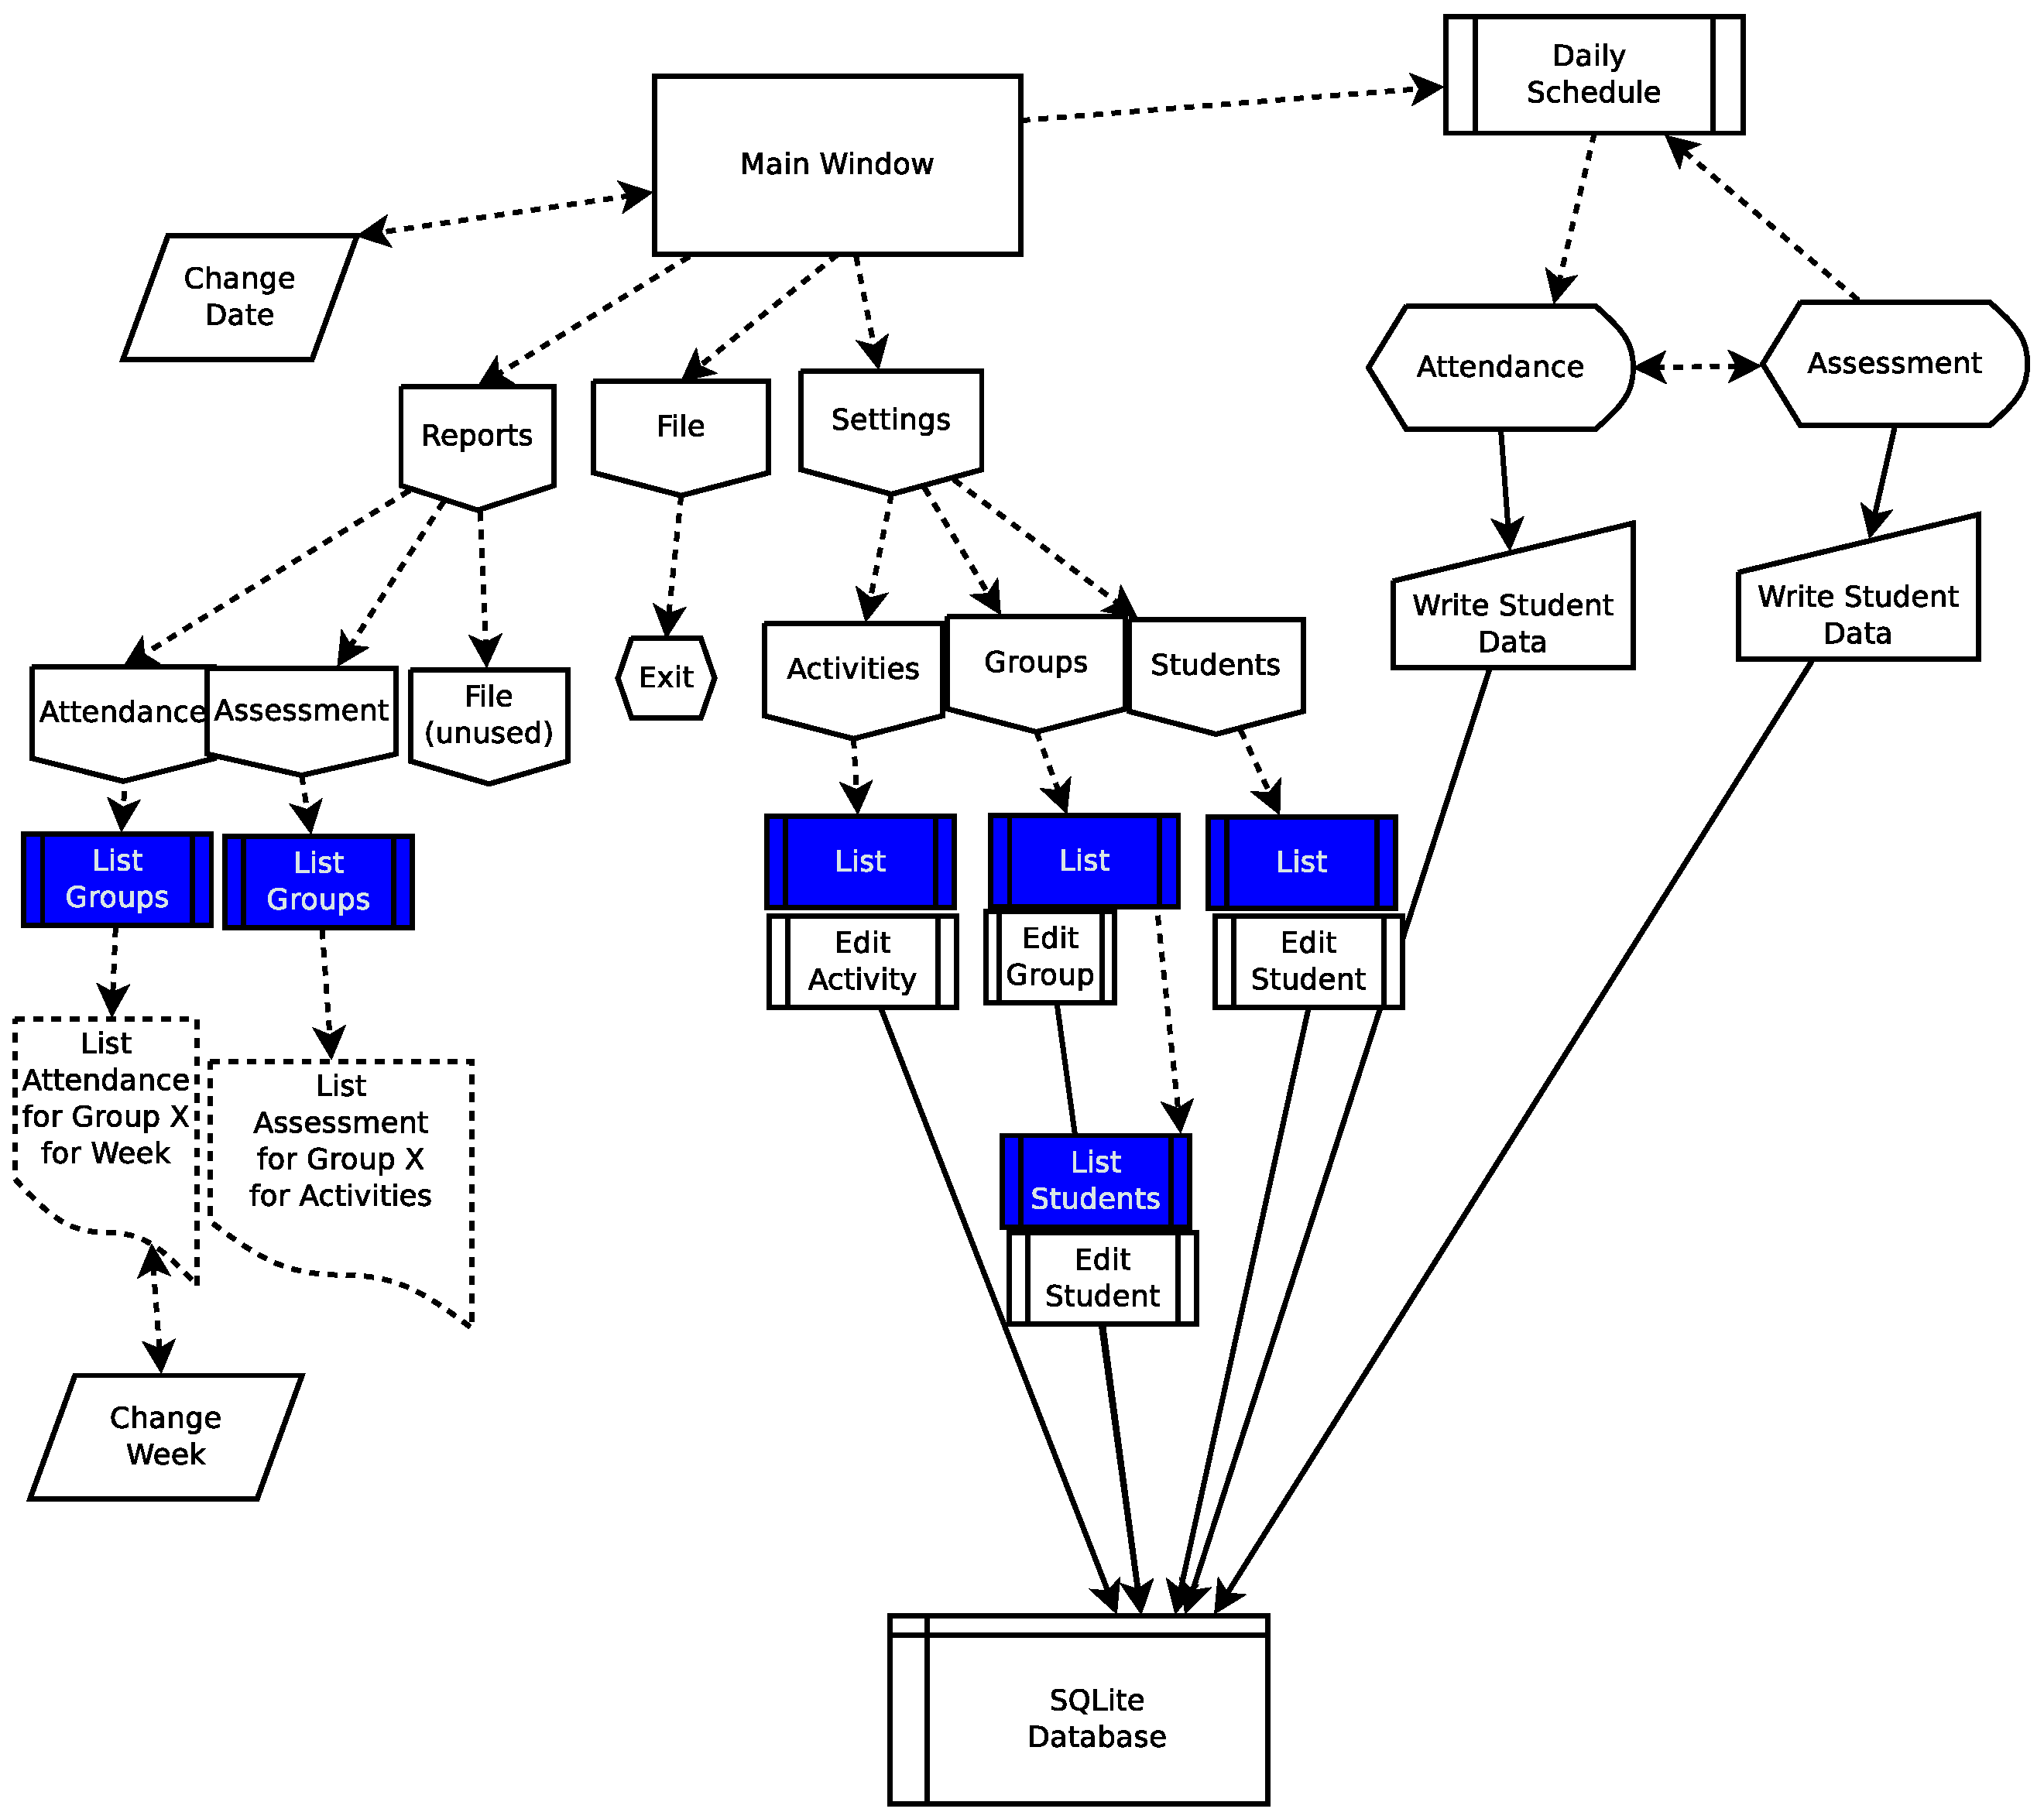
\includegraphics[scale=0.3]{eduxes_diagram.eps}
		        \caption{Diagram}
		        \label{fig:diagram}
		    \end{center}
		\end{figure}
		
